% This LaTeX template is intended for the students of CSI\index{SI} Master from
% University of Bordeaux to make their reports.
%
% This template can be used and modified with no restriction.
%
% %%% History %%%
%
% * April 22, 2014: First version (Emmanuel Fleury <fleury@labri.fr>)
% * May 09, 2016 First realase (Rémi Tremblain <remi.tremblain@soprasteria.com>)
%
% 
%

\documentclass[a4paper]{memoir}

\setcounter{tocdepth}{3}
\setcounter{secnumdepth}{3}

%%%%% Packages %%%%%
\usepackage{lmodern}
\usepackage{palatino}
\usepackage[T1]{fontenc}
\usepackage[utf8]{inputenc}

% To be removed if you want it in english
\usepackage[french]{babel}

\usepackage{amstext,amsmath,amssymb,amsfonts}
\usepackage{multirow,colortbl}
\usepackage{xspace,varioref}
\usepackage{hyperref}


\usepackage[dvipsnames]{xcolor}
\usepackage{graphicx}
\usepackage{appendix}
\usepackage{makeidx} 
\usepackage{csquotes}


%% custom style %%%%%%%%%%%%%%%%%%%%%%%%%%%%%%%%%%%%%%%%%%%%%%%%%%%%%%%%

% custom commands
\newcommand{\version}[1]{\def\theversion{#1}}
\newcommand{\subtitle}[1]{\def\thesubtitle{#1}}

\newcommand{\authors}[1]{\def\theauthors{#1}\author{#1}}
\newcommand{\supervisor}[1]{\def\thesupervisor{#1}}
\newcommand{\tutor}[1]{\def\thetutor{#1}}

% translation for custom words
\newcommand{\authorname}{Author}
\newcommand{\authorsname}{Authors}
\newcommand{\supervisorname}{Supervisor}
\newcommand{\tutorname}{Tutor}

\newcommand{\thepartname}{Part}

\ifdefined\addto{%
\addto{\captionsfrench}{\renewcommand{\authorname}{Auteur}}%
\addto{\captionsfrench}{\renewcommand{\authorsname}{Auteurs}}%
\addto{\captionsfrench}{\renewcommand{\supervisorname}{Superviseur}}%
\addto{\captionsfrench}{\renewcommand{\tutorname}{Tuteur}}}
\addto{\captionsfrench}{\renewcommand{\thepartname}{Partie}}
\else{}
\fi

%%%%% Setting Titlepage %%%%%
%%%%%%%%%%%%%%%%%%%%%%%%%%%%%
\pretitle{\flushleft\Huge\textsf}
\posttitle{\\[-.65em]\rule{\linewidth}{1.5mm}\\[-.65em]
\ifx\thesubtitle\undefined%
\else%
\hfill{\small\itshape \thesubtitle}%
\fi
\centering
\vfill

\includegraphics{Universite_de_Bordeaux.pdf}
\vfill
\iflanguage{french}{%
{\Huge\bfseries Mémoire de fin d'étude}
% {\Huge Projet de deuxième année}
% {\Huge Projet de première année}
}{%
{\Huge Master Thesis}
% {\Huge Master2 Project}
% {\Huge Master1 Project}
}\\
\vspace{1.25em}
\iflanguage{french}{%
\LARGE
Master \emph{Sciences et Technologies},\\
Mention \emph{Informatique},\\
% Mention \emph{Mathématiques},\\
Parcours \emph{Cryptologie et Sécurité Informatique}.\\
\par\hfill%
}{%
\LARGE
Master in \emph{Sciences and Technologies},\\
Specialty in \emph{Computer Science},\\
% Specialty in \emph{Mathematics},\\
Track \emph{Cryptology and Computer Security}.\\
\par\hfill
}}

%% author
\preauthor{\vspace{\fill}\\
\ifx\theauthors\undefined%
\flushleft\textbf{\large\authorname}\\
\else%
\flushleft\textbf{\large\authorsname}\\
\fi
\small}
\postauthor{\vspace{1em}
\ifx\thesupervisor\undefined%
\else%
\newline\textbf{\large\supervisorname}\\\thesupervisor\\[1em]%
\fi
\ifx\thetutor\undefined%
\else%
\textbf{\large\tutorname}\\\thetutor%
\fi
\\[-.25em]
\rule{\linewidth}{1mm}\\[-.25em]}

%% version and date
\predate{\hspace{\fill}
\ifx\theversion\undefined%
\else%
version~\theversion~--~%
\fi}
\postdate{}

%% chapters style %%%%%%%%%%%%%%%%%%%%%%%%%%%%%%%%%%%%%%%%%%%%%%%%%%%%%%
%% You may try several styles (see more in the memoir manual).

\chapterstyle{veelo}
%\chapterstyle{chappell}
%\chapterstyle{ell}
%\chapterstyle{ger}
%\chapterstyle{pedersen}
%\chapterstyle{verville}
%\chapterstyle{madsen}
%\chapterstyle{thatcher}

%% parts style %%%%%%%%%%%%%%%%%%%%%%%%%%%%%%%%%%%%%%%%%%%%%%%%%%%%%%%%%

\renewcommand*{\thepart}{\arabic{part}}

\renewcommand*{\parttitlefont}{\chaptitlefont\Huge}
\renewcommand*{\partnamefont}{\chapnamefont\HUGE}
\renewcommand*{\partnumfont}{\chapnumfont\HUGE}

\renewcommand{\beforepartskip}{\vspace*{\fill}}
\renewcommand{\midpartskip}{\vspace{.5em}\hrule height 1.5mm \vspace{.5em}}
\renewcommand{\afterpartskip}{\vspace*{\fill}}

% table of contents
\renewcommand*{\cftpartname}{\thepartname}
\renewcommand*{\cftpartpresnum}{\space}
\renewcommand*{\cftpartaftersnum}{.}
\renewcommand*{\cftpartaftersnumb}{\space}

\cftpagenumbersoff{part}
\renewcommand{\cftpartafterpnum}{\protect\\[-.75em]%
\protect\mbox{}\protect\hrule\par}

\renewcommand{\cftchapterdotsep}{4}


%% index generation %%%%%%%%%%%%%%%%%%%%%%%%%%%%%%%%%%%%%%%%%%%%%%%%%%%%
\makeindex

%%%%% Useful macros %%%%%
\newcommand{\latinloc}[1]{\ifx\undefined\lncs\relax\emph{#1}\else\textrm{#1}\fi\xspace}
\newcommand{\etc}{\latinloc{etc}}
\newcommand{\eg}{\latinloc{e.g.}}
\newcommand{\ie}{\latinloc{i.e.}}
\newcommand{\st}{\ensuremath{\text{\xspace s.t.\xspace}}}


%%%%% Report Title %%%%%
\title{Audit technique et pentest}
\subtitle{Etat de l'art, situation et évolution}

% If only one author use \author
\author{Rémi Tremblain \texttt{<remi.tremblain@etu.u-bordeaux.fr>}}

% If several authors use \authors{}
%\authors{Jean Dupont \texttt{<jean.dupont@etu.u-bordeaux.fr>}\\
%Stéphanie Martin \texttt{<stephanie.martin@etu.u-bordeaux.fr>}}

\supervisor{Pierrick Conord \texttt{<pierrick.conord@soprasteria.com>}}

\tutor{Emmanuel Fleury \texttt{<fleury@labri.fr>}}

%\version{0.1}

%%%%% Document %%%%%
%%%%%%%%%%%%%%%%%%%%
\begin{document}

\frontmatter%%%%%%%%%%%%%%%%%%%%%%%%%%%%%%%%%%%%%%%%%%%%%%%%%%%%%%%%%%%%
\maketitle
\thispagestyle{empty}

%%%%%%%%%%%%%%%%%%%%%%%%%%%%%%%%%%%%%%%%%%%%%%%%%%%%%%%%%%%%%%%%%%%%%%%%

\cleardoublepage
\par\vspace*{\fill}

\iflanguage{french}{%
\section*{Déclaration de paternité du document}
}{%
\section*{Declaration of authorship of the document}}

\ifx\theauthors\undefined%
\iflanguage{french}{%
  Je certifie sur l'honneur que ce document que je soumet pour
  évaluation afin d'obtenir le diplôme de Master en \emph{Sciences et
    Technologies}, Mention \emph{Informatique}, Parcours \emph{Cryptologie et Sécurité
    Informatique}, est entièrement issu de mon propre travail, que
  j'ai porté une attention raisonnable afin de m'assurer que son
  contenu est original, et qu'il n'enfreint pas, à ma connaissance,
  les lois relatives à la propriété intellectuelle, ni ne contient de
  matériel emprunté à d'autres, du moins pas sans qu'il ne soit
  clairement identifié et cité au sein de mon document.
  \bigskip

  \hfill\textbf{Date et Signature}
}{%
  I hereby certify that this material, which I now submit for
  assessment on the programme of study leading to the award of the
  Master in \emph{Sciences and Technologies}, Specialty in
  \emph{Mathematics} or \emph{Computer Science}, Track
  \emph{Cryptology and Computer Security}, is entirely my own work,
  that I have exercised reasonable care to ensure that the work is
  original, and does not to the best of my knowledge breach any law of
  copyright, and has not been taken from the work of others save and
  to the extent that such work has been cited and acknowledged within
  the text of my work.
  \bigskip

  \hfill\textbf{Date and Signature}}
\else%
\iflanguage{french}{%
  Nous certifions sur l'honneur que ce document que nous soumettons
  pour évaluation afin d'obtenir le diplôme de Master en
  \emph{Sciences et Technologies}, Mention \emph{Mathématiques} ou
  \emph{Informatique}, Parcours \emph{Cryptologie et Sécurité
    Informatique}, est entièrement issu de notre propre travail, que
  nous avons porté une attention raisonnable afin de nous assurer que
  son contenu est original, et qu'il n'enfreint pas, à notre
  connaissance, les lois relatives à la propriété intellectuelle, ni
  ne contient de matériel emprunté à d'autres, du moins pas sans qu'il
  ne soit clairement identifié et cité au sein de notre document.
  \bigskip

  \hfill\textbf{Date et Signatures}
}{%
  We hereby certify that this material, which we now submit for
  assessment on the programme of study leading to the award of the
  Master in \emph{Sciences and Technologies}, Specialty in
  \emph{Mathematics} or \emph{Computer Science}, Track
  \emph{Cryptology and Computer Security}, is entirely our own work,
  that we have exercised reasonable care to ensure that the work is
  original, and does not to the best of our knowledge breach any law
  of copyright, and has not been taken from the work of others save
  and to the extent that such work has been cited and acknowledged
  within the text of our work.\bigskip

  \hfill\textbf{Date and Signatures}}
\fi
\vspace{6em}


%%%%%%%%%%%%%%%%%%%%%%%%%%%%%%%%%%%%%%%%%%%%%%%%%%%%%%%%%%%%%%%%%%%%%%%%

\chapter*{Résumé}

\index{Résumé}

Le monde de la sécurité informatique est en constante évolution et nous voyons aujourd'hui l'avancement de ce domaine.
Ce domaine est considéré comme un point important dans le développement d'une entreprise et sa nécessité n'est aujourd'hui plus à discuter à mesure que le temps passe. En effet, peu importe la taille de l'infrastructure ou les données qu'elle traite, l'entreprise utilise dans la quasi-totalité du temps du Système d'information\index{Système d'information}. Et qui dit matériel informatique dit sécurité informatique. Ceci passe par la mise en place de standard, de règle, de formation ou encore de sensibilisation du personnel mais elle reste souvent source de problème dans les entreprises, l'actualité quotidienne sur le sujet faisant foi.\\

L'informatique reste un domaine de plus en plus important, ne serait-ce que dans notre quotidien, de nombreuse activé en dépendent. Cela se remarque également par le nombre d'objet connecté qu'il existe et de la facilité d'accès à l'informatique. De ce fait, la sécurité informatique se doit de suivre ce développement rapide de l'informatique. Mais d'où vient cette nécessité ? Pourquoi est-il nécessaire désormais de prévoir du budget dans la sécurisation du matériel informatique dans une entreprise ? On peut bien-sûr pointer l'avancer rapide de l'informatique et sa démocratisation et par conséquent l'évolution des besoins en terme de sécurisation. En effet, au début de l'apparition de l'informatique, on réalisait une forme de sécurité par le dégât, autrement dit, on sécurisait les systèmes après avoir subi une attaque, parce que la mentalité des pirates n'était pas la même par exemple.
Mais depuis les années 2000, avec l'explosion de la bulle internet et de son accès facilité, la notion de sécurité informatique devient importante et de nombreux standards voient le jour afin de répondre à la demande croissante de sécurisation.

Nous allons essayer de voir cela dans ce rapport, ce qui rendra une étude de ce qu'il existe en terme de prestation de sécurité informatique, pourquoi nous en sommes arrivés ici et qu'elles sont les possibilités futures.


%%%%%%%%%%%%%%%%%%%%%%%%%%%%%%%%%%%%%%%%%%%%%%%%%%%%%%%%%%%%%%%%%%%%%%%%

\chapter*{Présentation de l'entreprise}

Ce travail a été effectué dans le cadre du stage de fin d'étude qui se déroulait sur une période de six mois, au sein de la société Sopra Steria\index{Sopra Steria}.
Les informations qui suivent sont une présentation de la société, de son organisation ainsi que son activité.

\section*{Historique}

En janvier 2015, Sopra et Steria ont choisi de s’unir dans le groupe Sopra Steria\index{Sopra Steria}. Ils disposent d’une histoire et d’une culture proches : pionniers des services informatiques, ils se sont bâtis sur une forte culture entrepreneuriale et d’innovation.

Grâce à de très fortes complémentarités des métiers et des géographies, le nouvel ensemble propose l’une des offres les plus complètes du marché, répondant au mieux aux attentes du client. 

\begin{figure}[!ht]
\center
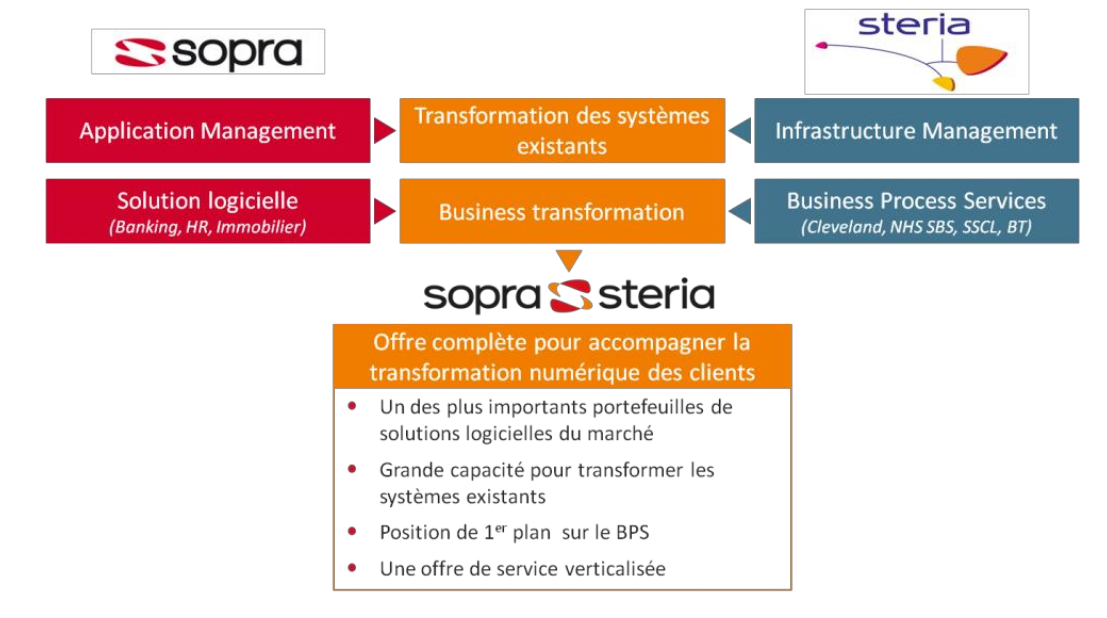
\includegraphics[width=1\textwidth]{./images/sopra1.png}
\caption{Fusion Sopra \& Steria}
\label{Sopra+Steria}
\end{figure}

Sopra Steria\index{Sopra Steria} est un leader européen de la transformation numérique. Le groupe se positionne dans le top 4 en France et dans le top 10 en Europe des sociétés de services IT (source Gartner).

\newpage

\begin{figure}[!ht]
\center
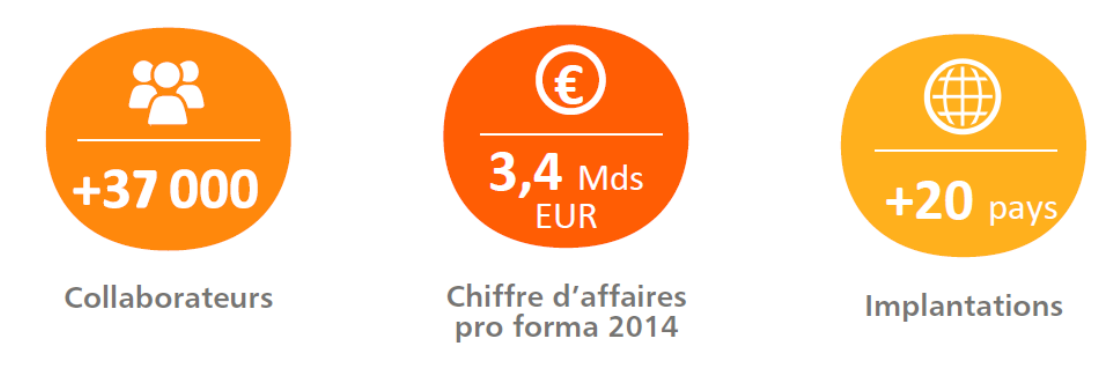
\includegraphics[width=1\textwidth]{./images/sopra2.png}
\caption{Valorisation}
\label{Sopra+Steria+chiffre}
\end{figure}

Avec un CA de près de 3,4 Milliards d’euros (proforma) en 2014, Sopra Steria\index{Sopra Steria} est localisé dans plus de 20 pays à travers le monde, principalement en Europe.
La révolution du numérique est une source d’opportunités pour leur clients dans leur transformation et la fourniture de service de qualité tout en maîtrisant cet écosystème IT ainsi que son coût.

\begin{figure}[!ht]
\center
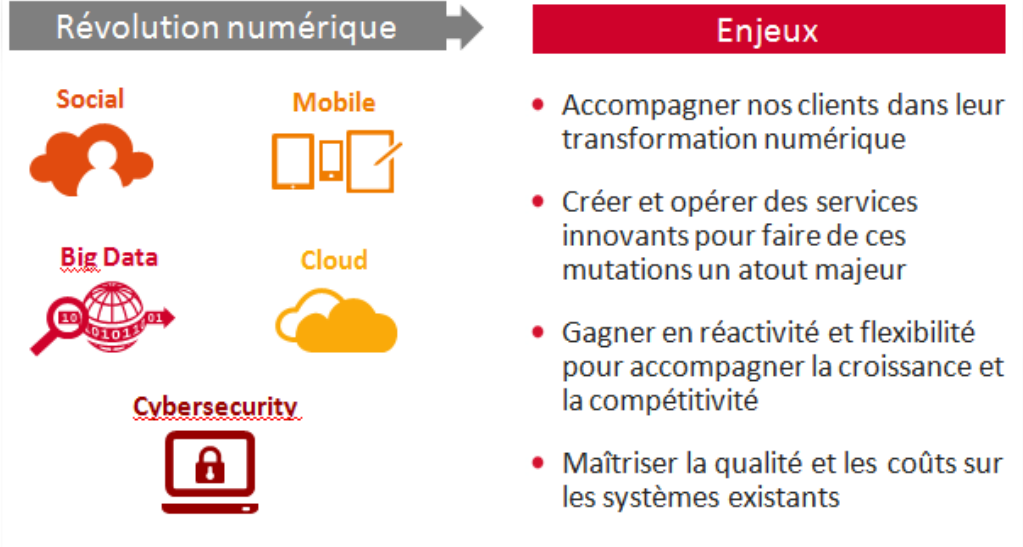
\includegraphics[width=1\textwidth]{./images/sopra3.png}
\caption{Révolution numérique}
\label{Révolution numérique}
\end{figure}

Sopra Steria\index{Sopra Steria} intervient sur l’ensemble des prestations d’accompagnement dans la réalisation de vos projets.
Nos savoir-faire forment une chaîne continue de valeur ajoutée, du conseil Métier / SI\index{SI} à la gestion d’infrastructure en passant par l’intégration de système et la gestion d’applications.

\newpage

\section*{Activité}

L’ensemble de l’expertise de Sopra Steria\index{Sopra Steria} est regroupé au sein de la filiale Solutions \& Cyber dans une BU CyberSécurité sous la responsabilité d’Ilhame CHOUKRANI.

\begin{figure}[!ht]
\center
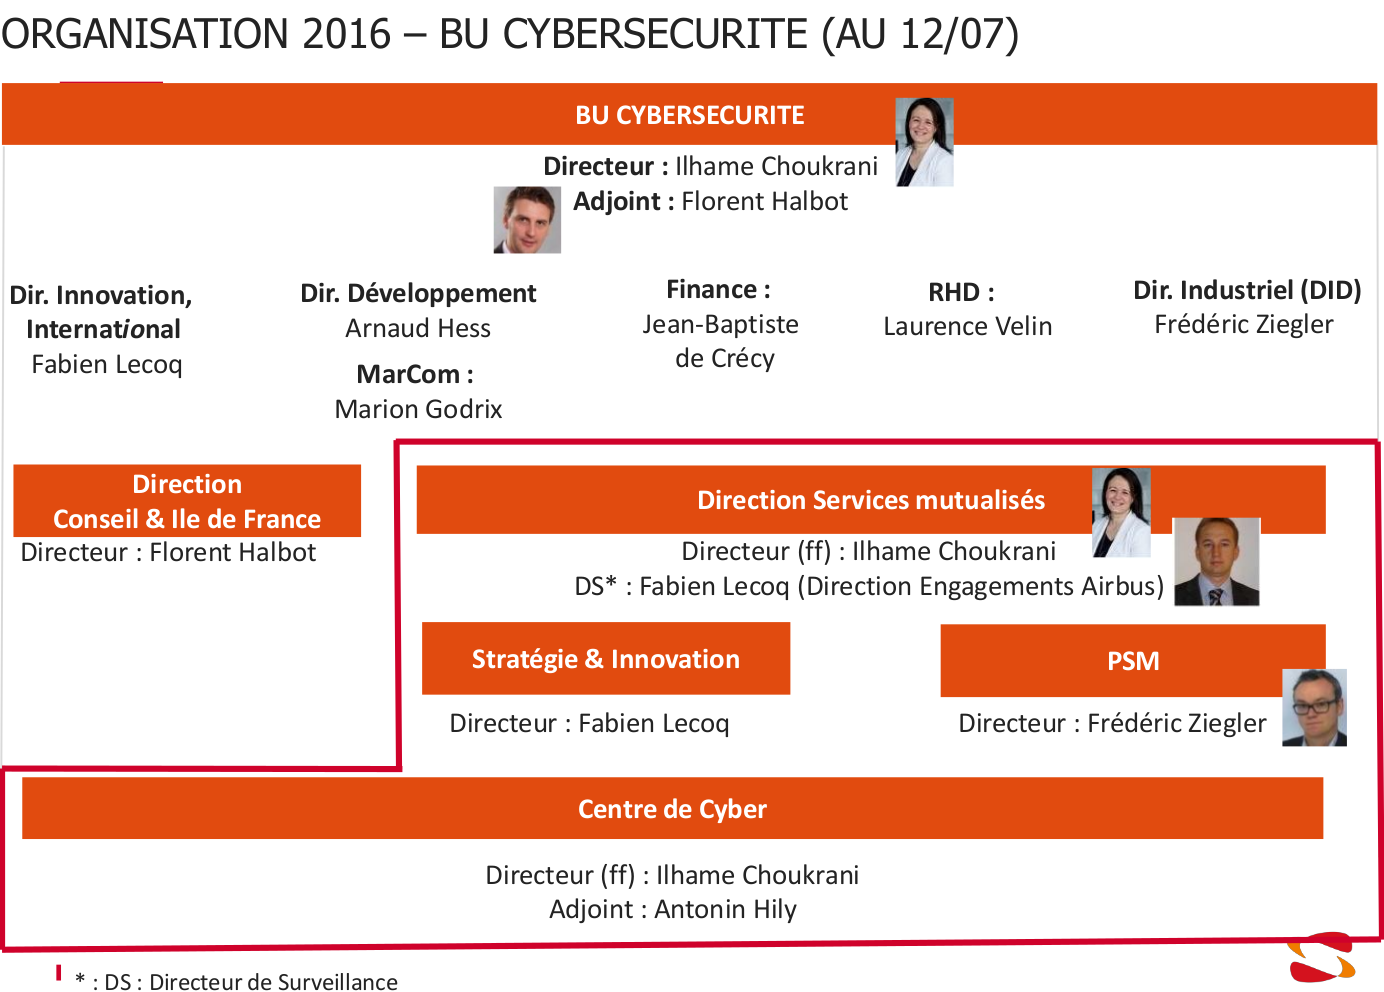
\includegraphics[width=1\textwidth]{./images/sopra4.png}
\caption{Organigrame}
\label{Organigrame}
\end{figure}

Cette Business Unit compte : 

\begin{itemize}
\item Plus de 200 consultants, experts SSI\index{SI} en France ;
\item 3 Centres de CyberSécurité (France, UK et Singapour) ;
\item Un budget R\&D d'environ 3,3\% du CA Sécurité.
\end{itemize}

Carte d’identité de la BU CyberSécurité et chiffres clés dans le monde :

\begin{figure}[!ht]
\center
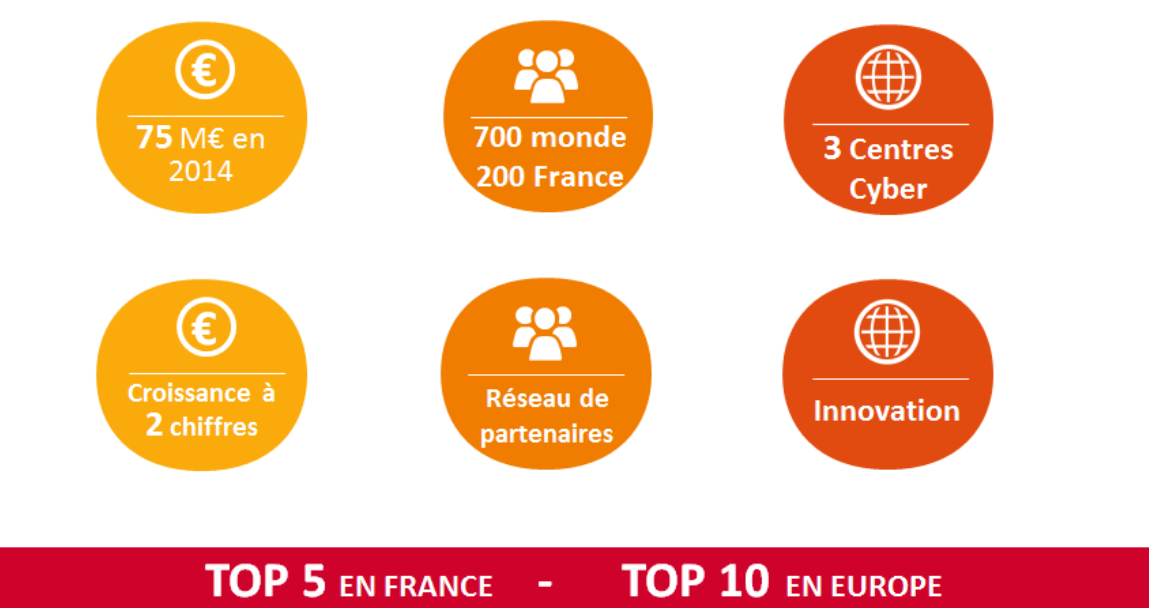
\includegraphics[width=0.8\textwidth]{./images/sopra5.png}
\caption{Carte d'identité}
\label{ID}
\end{figure}

\cleardoublepage
\tableofcontents*

%%%%%%%%%%%%%%%%%%%%%%%%%%%%%%%%%%%%%%%%%%%%%%%%%%%%%%%%%%%%%%%%%%%%%%%%

\mainmatter%%%%%%%%%%%%%%%%%%%%%%%%%%%%%%%%%%%%%%%%%%%%%%%%%%%%%%%%%%%%%


\chapter*{Introduction}

Le secteur de la sécurité informatique connait une croissance importante depuis les années 90, de par son importance dans les entreprises et la démocratisation de l'informatique tout public. On retrouve en effet l'informatique dans toutes ses formes à tous les niveaux de l'industrie, par la gestion d'informations plus ou moins sensibles, mais aussi chez les particuliers désireux d'explorer un monde informatique qui évolue très rapidement.\\

Cependant, une faible proportion des utilisateurs d'éléments informatiques (internet, ordinateur, etc.) est correctement sensibilisée à la bonne pratique de ces derniers. Et c'est ici le commencement de la réflexion sur lequel ce rapport se porte. En effet, si l'informatique se démocratise, il est important d'en connaitre les bonnes pratiques, les enjeux et risques que ce développent rapide provoque et plus particulièrement sur l'aspect de la sécurisation informatique dite industrielle.

Nous allons donc aborder ce mémoire de façon chronologique, avec, dans un premier temps, un état de l'art de la sécurisation informatique, en expliquant les prémices de l'informatique et de la sécurisation informatique. Nous discuterons dans cette même partie de l'aspect théorique de la sécurisation informatique comme notamment ce qu'il est nécessaire de sécuriser ou pourquoi sécuriser telle ou telle information.
Dans un second temps, pour aborder plus un aspect actuel de la sécurité, nous partirons sur une partie dite technique en expliquant ce qu'il existe de nos jours en termes d'outils, de prestation ou de modèle pour cadrer et mettre en place une sécurisation informatique appliquée à l'industrie. Nous parlerons aussi du cadre juridique qu'il est nécessaire de mettre en place pour exercer ce genre d'activité. Enfin, pour aborder le futur de la sécurité informatique, nous nous dirigerons vers les modèles qui tendent à immerger, l'évolution des pratiques ou encore l'ouverture au grand public.\\

Dans ce mémoire, l'auteur se basera sur sa vision de la sécurité informatique dite industrielle à travers la société Sopra Steria\index{Sopra Steria}, productrice de service de sécurisation informatique, et de son ouverture au niveau international.



%%%%%%%%%%%%%%%%%%%%%%%%%%%%%%%%%%%%%%%%%%%%%%%%%%%%%%%%%%%%%%%%%%%%%%%

\part{Etat de l'art \& aspect théorique}


\chapter{Etat de l'art}%%%%%%%%%%%%%%%%%%%%%%%%%%%%%%%%%%%%%%%%%%%%%%%%%%%%%%%%%%%%%%%%%%%%%%%

Dans cette partie, nous aborderons la question du ``Pourquoi'', en expliquant les origines de la sécurité informatique, les idées reçues sur cette discipline aussi nouvelle qu'incomprise et pourquoi elle est aujourd'hui estimée comme un aspect primordial, voire obligatoire, dans le développement d'une entreprise.

\noindent Mais si nous devons parler de l'état actuel de la sécurité informatique, il est important de parler de ses origines, nous nous intéresserons donc dans un premier temps au développement de l'informatique lui-même en établissant un état de l'art. Pour cela, nous allons expliquer à travers différents moments clés de l'histoire qui ont permis la naissance et le développement de l'informatique tel que nous le connaissons aujourd'hui.\\


\section{Enigma}

Impossible de parler de sécurité informatique sans parler de cette invention faite par des cryptographes polonais en 1918 : Enigma\index{Enigma}.
À l'origine, ce dispositif électromécanique de chiffrement par rotor fut inventé pour sécuriser les communications bancaires, mais l'armée allemande en trouve une utilité tout autre en s'en servant pour sécuriser ses communications durant la seconde guerre mondiale. Mais le plus important dans cette invention fut été la réponse faite par les alliées, avec l'aide d'Alan Turing\index{Alain Turing}\footnote{Mathématicien et cryptologue britannique né en 1912 et mort en 1954, auteur de travaux qui fondent scientifiquement l'informatique} avec la création de la machine Colossus\index{Colossus}\footnote{Premier calculateur électronique fondé sur le système binaire} pour briser les codes provenant d'Enigma\index{Enigma}. On accrédite d'ailleurs la fin de la guerre d'une année plus tôt à cette machine.

On voit donc à partir de cette date, l'apparition de ce que l'on pourrait appeler le premier ordinateur, ouvrant ainsi la porte à l'informatique moderne.

\section{Les années 60 \& ARPANet\index{ARPANet}}

On se place désormais dans les années 60, au moment du commencement de l'industrialisation des ordinateurs grand public. Mais cette période apporte son lot d'avancements en matière de sécurité informatique et nous allons comprendre pourquoi avec quelques faits historiques marquants.\\

Un des points importants de l'évolution de l'informatique se passe avec un groupe d'étudiants du MIT\footnote{Massachusetts Institute of Technology} qui, vers 1959, fonde le Tech Model Railroad Club (TMRC) afin d'obtenir l'accès a ce que l'on appellera aujourd'hui le premier ordinateur industriel : le PDP-1. À travers leur club ils commencèrent à étudier, explorer et coder sur cette unité centrale et mettent au point le premier jeu vidéo sur micro-ordinateur : Spacewar\index{Spaceware!}. Mais ce n'est pas le plus important fait relayé à ce club, en effet on lui attribuera la naissance du terme ``hack'' et de tous ses dérivés, mais aussi tout un jargon qui fait maintenant partie du Jargon File\footnote{Glossaire spécialisé dans l'argot des programmeurs}.\\

Le fait le plus marquant dans l'évolution de l'informatique se passe en 1969 avec un projet mené le Ministère de la Défense américaine (DoD) : le réseau Advanced Research Projects Agency Network (ARPANet\index{ARPANet}). Ce projet permettra de relier quatre universités américaines à travers les États-Unis grâce à un concept de transfert de paquets, qui deviendra par la suite la base du transfert de données sur internet. L'intérêt de cette avancée se situait sur le fait que les communications étaient basées sur la communication par circuits électronique, telle que celle utilisée par le réseau téléphone, où un circuit dédié est activé lors de la communication avec le poste du réseau. Mais avec le réseau développé par la DARPA\index{DARPA}, on met en avant une communication plus robuste et capable d'être établie sur de plus grande distance. Il a été en effet développé dans le but de continuer à fonctionner malgré une attaque nucléaire massive de la part de l'Union soviétique (contexte de la guerre froide) et permettant à un paquet émis d'adapter son chemin en fonction de l'état du réseau (changement de noeud, etc.)

Enfin, on ne peut parler des années 60 sans parler du développement d'UNIX\index{UNIX} par Ken Thompson, considéré par beaucoup comme étant le système d'exploitation le plus ``susceptible d'être piraté'' en raison d'une part, de ses outils pour développeurs et de ses compilateurs très accessibles et d'autre part, de son soutien parmi la communauté des utilisateurs. À peu près à la même époque, Dennis Ritchie met au point le langage de programmation C, indiscutablement le langage de piratage le plus populaire de toute l'histoire informatique.\\

On peut donc penser que cette époque apporte son lot d'évènements majeurs dans le développement de l'informatique, de par le jargon mis en place et très largement utilisé de nos jours, mais aussi par l'environnement UNIX\index{UNIX} qui a vu le jour et le langage de programmation le plus utilisé aujourd'hui. Mais le plus gros impact de cette décennie reste la mise en place du réseau ARPANet\index{ARPANet}, ancêtre de l'internet, mais qui se positionne comme étant un moyen d'échanger des données sur un réseau et ce, sans se préoccuper de la distance. Il restera cependant limité aux universités et professionnel dans ses premières versions.

\section{Les années 70}

Les années 70 quant à elles, sont importantes pour la démocratisation de l'informatique pour le grand public en palliant aux problèmes d'accès au réseau de données ARPANet\index{ARPANet}. En effet, la société Bolt, Beranek et Newman, met au point le protocole de communication Telnet\footnote{TErminal NETwork ou TELecommunication NETwork, ou encore TELetype NETwork} comme étant une extension publique du réseau ARPANet\index{ARPANet}, cassant ainsi le privilège des entrepreneurs et des chercheurs du monde académique quant à son accès. Ce protocole ouvre donc la voie à l'utilisation du réseau de données pour le grand public. Mais cependant, l'accès au matériel informatique nécessaire pour l'accès au réseau reste compliqué. C'est sur ce point que Steve Jobs et Steve Wozniak créent Apple Computer, et mettant ainsi au point et commercialisant le premier ordinateur personnel ou PC (de l'anglais Personal Computer). Le PC devient alors un accélérateur dans l'apprentissage par des utilisateurs malintentionnés de l'art de s'introduire dans des systèmes à distance en utilisant du matériel de communication de PC courant que des modems analogues ou des logiciels dédiés (war dialers\index{War Dialers}). Comme la sécurité telle que nous la connaissons actuellement n'existait pas, il était d'autant plus facile de trouver et d'exploiter des vulnérabilités sur les systèmes informatiques.\\
\noindent On peut aussi noter l'apparition d'un système de messagerie pour la communication électronique entre des utilisateurs très variés. USENET, crée par Jim Ellis et Tom Truscott, devient rapidement l'un des forums les plus populaire pour l'échange d'idées en matière de tout et n'importe quoi, mais principalement d'informatique, de mise en réseau et bien évidemment, de piratage.\\
C'est dans cette période-là que la nécessité de sécurité informatique commence à se faire ressentir, puisque l'accès à l'information commence à être de plus en plus facile et de plus en plus dangereuse étant donné que les standards de contrôle ne sont pas encore mis en place et que ce domaine reste assez récent.


\section{Années 80}

Dans les années 80, IBM\footnote{International Business Machines Corporation} fait une avancée en matière d'équipement informatique en produisant des ordinateurs basés sur le microprocesseur Intel 8086. Ce processeur à faible coût permet à l'informatique de passer d'une utilisation purement professionnelle à une utilisation personnelle, et cela permet à l'ordinateur de devenir un produit ménager de consommation courante. Ce changement de situation permet de rendre le PC plus abordable, puissant mais aussi plus simple d'utilisation et contribue à une prolifération de ce matériel dans l'environnement professionnel et personnel, et par conséquent dans celui d'utilisateurs malintentionnés.

Mais avec ce développement soudain de l'informatique et de ses mauvaises pratiques, le monde fait face à une recrudescence de des délits informatiques, notamment avec les deux groupes pionniers en matière de piratage informatique qui commencent à se faire remarquer dans leur exploitation des faiblesses des ordinateurs et des réseaux de données électroniques : Legion of Doom et Chaos Computer Club. Mais un constat rapide est dressé : la loi n'est pas suffisamment armée pour faire face à cette nouvelle tendance. Ce n'est qu'en 1986 que le congrès américain vote une loi sur la répression des fraudes et des infractions dans le domaine informatique\footnote{Computer Fraud and Abuse act} à la suite des exploits de Ian Murphy, plus connu sous le nom de Captain Zap, qui réalisa l'exploit de s'introduire dans les ordinateurs de l'armée pour voler des informations des bases de données de commandes de diverses sociétés et utiliser des standards téléphoniques gouvernementaux à accès limités pour effectuer des appels personnels. 
Cette avancement en matière de juridiction met donc l'accent sur la dangerosité de l'informatique et sur la nécessité de cadrer ce qui s'en rapporte et donc, par conséquents de la nécessité de la sécurité informatique.

Paradoxalement, pour faire suite à l'augmentation des menaces informatiques et par crainte que le « ver Morris »\footnote{En référence à son créateur Robert Morris, un diplômé universitaire qui infectât pas moins de 6000 machines relié à l'internet.} puisse être reproduit, l'équipe de réponse aux urgences informatiques (CERT\index{CERT}, de l'anglais Computer Emergency Response) est créée afin d'avertir les utilisateurs d'ordinateurs contre les problèmes de sécurité réseau.

On voit donc apparaitre dans les années 80 les réponses aux problèmes informatiques modernes de par les institutions qui émergent mais aussi par la réglementation qui s'impose pour faire face aux nouvelles menaces.

\section{Année 90}

La période des années 90 est la plus intéressante pour le développement de notre mémoire. C'est celle-ci qui marque les plus grandes avancées dans le domaine de l'informatique et de sa sécurité.
Commençons avec le fait plus marquant de cette période avec la dé-commission de l'ARPANet\index{ARPANet} et le transfert de son trafic vers le World Wide Web\index{World Wide Web} tel que nous le connaissons aujourd'hui. C'est avec ce transfert que le premier navigateur Web graphique voit le jour : WordlWideWeb. Cette innovation engendrant une croissance exponentielle de la demande pour l'accès public à l'internet. Avec cette explosion de l'internet, les délits se multiplient, comme nettement avec Kevin Mitnick, considéré comme le plus célèbre de tous les pirates, pour s'être introduit dans les systèmes de plusieurs grandes sociétés et avoir volé toute sorte de données allant des informations personnelles de personnes célèbres à plus de 20.000 numéros de cartes de crédit en passant par l'extraction de code source de logiciels propriétaires \\
\noindent C'est par la même occasion que le ministre de la justice américaine, Attorney General Janet Reno, en réponse au nombre croissant des brèches de sécurité dans les systèmes du gouvernement fonde le centre de protection de l'infrastructure nationale (ou National Infrastructure Protection Center, NIPC).


\section{De nos jours}

Entre les années 1990 et 2000, le nombre d'ordinateurs est passé d'un million à plus de 370 millions, la barre du milliard de sites web a même été franchie en 2014. L'accès à l'informatique et internet s'est vu banalisé, au même titre que l'accès à du contenu de nature controversé, comme avec des ressources sur le darknet\footnote{Réseau privé virtuel anonymisé} ou les forums de discussions décentralisés.
Cependant, avec toutes ces activités, le nombre d'incident augmente et tous les jours, environ 225 cas majeurs de brèches de sécurité sont rapportés au Centre de Coordination du CERT\index{CERT} à l'université de Carnegie Mellon.
En 2003, le nombre d'infractions rapporté au CERT\index{CERT} est monté à 137.529, par rapport à 82.094 en 2002 et par rapport à 52.658 en 2001
L'impact économique au niveau mondial des trois virus Internet les plus dangereux ayant surgi au cours des trois dernières années a atteint un montant total d’US \$13,2 milliards\\

On voit donc bien avec ce développement historique de l'informatique et de ses besoins en matière de sécurité informatique, notamment pour les industries, pour qui la sécurité fait désormais partie des dépenses non seulement quantifiables, mais justifiables incluses dans tout budget. Les sociétés nécessitant de l'intégrité et la haute disponibilité de données recourent aux capacités des administrateurs système, développeurs et ingénieurs pour assurer la fiabilité de leurs systèmes, services et informations 24 heures sur 24, 7 jours sur 7. La possibilité de devenir la victime d'attaques coordonnées, d'utilisateurs ou de processus malveillants représente une véritable menace au succès d'une société. 

\chapter{Aspect théorique}

La sécurité de l'information et de la sécurité informatique en général est soumise à des contraintes particulières car elle s'appuie essentiellement sur la bonne coopération de l'utilisateur. Car de nos jours, 90\% des problèmes de sécurité informatique sont dûs à une négligence humaine.\\
La question légitime qu'il serait bon de se poser serait de savoir ce que l'on doit sécuriser. Ce à quoi on pourrait répondre ``tout''. Mais la sur-sécurisation reste un problème dans le sens où elle est beaucoup trop compliquée à mettre en place de par la multitude d'information disponible, la complexité de la tâche et de la mise en place, l'intrusivité et la bienveillance de l'utilisateur. Car la sécurité informatique n'est pas réservée à une élite formatée dans le domaine, elle passe avant tout par l'utilisateur lambda.\\
De nos jours, la mise en place de sécurité informatique passe par un raisonnement et un travail sur l'utilisateur et ce afin qu'elle soit le plus efficace possible. Elle ne doit pas être trop intrusive (pop-up, demande d'autorisation, UAC\footnote{User Access Control de Microsoft}, etc), trop envahissante ou trop compliquée pour que son utilisation soit la plus intuitive possible et faire en sorte qu'elle soit naturelle par l'utilisateur.\\

Un autre problème est qu'avant les années 2000, la sécurisation par le risque était très peu mis en œuvre : on sécurisait les endroits où l'on était attaqué. On pourrait appeler ça une sécurisation par "le dégât", étant donné que l'attaque a déjà eu lieu.
On y oppose à cette forme de sécurisation, la sécurisation par le risque. Elle s'effectue par la réalisation des analyses de risques et en sécurisant les éléments essentiels, les "organes vitaux" du système.

Nous allons donc voir dans la partie suivante ce dont on dispose pour réaliser la mise en place de toute la sécurité informatique, des outils mais aussi des méthodologies à notre disposition pour être actif et efficient.

%%%%%%%%%%%%%%%%%%%%%%%%%%%%%%%%%%%%%%%%%%%%%%%%%%%%%%%%%%%%%%%%%%%%%%%%
\part{Situation technique}

\chapter{Prémices}

La sécurité informatique est aujourd'hui quelque chose de très important dans le développement d'une entreprise, comme nous l'avons vu dans la partie précédente. Nous allons voir dans cette partie ce qu'il existe en terme d'outils et de prestation dans le monde de la sécurité informatique, en se penchant d'avantage sur la mise en oeuvre de test d'intrusion (ou pentest\index{Pentest}) et sa valeur vis à vis d'un audit de sécurité standard. Nous ferons le lien entre la partie précédente pour voir et constater si l'on est ou pas en mesure de répondre aux menaces en matière d'informatique. Nous verrons aussi par la suite tout ce qui touche au cadre légale et juridique, car, les différentes formes de sécurité (offensive\footnote{pentest\index{Pentest}} et défensive\footnote{Audit technique\index{Audit technique}}) doit être cadrée pour ne pas nuire à l'audité, ce qui serait contre-productif. On verra également la valeur ajoutée des CERT\index{CERT}ifications et des normes ISO qui fleurissent actuellement et leurs effets sur les prestations que les entreprises peuvent proposer et pourquoi elles deviennent de plus en plus nécessaires.\\ 

En terme de technique, nous allons voir ce qu'il existe en terme d'outillage pour réaliser les audits techniques (et ses variantes) et plus particulièrement les tests d'intrusions et les méthodologies qui y sont liées.\\
Mais commençons par distinguer tests d'intrusion et audit de sécurité, car il s'agit de deux notions qui peuvent paraître similaires au premier abord mais dont les cadres respectifs ne correspondent pas forcément et dont il est important de faire une différence. 
Un audit de sécurité est plus large qu'un test d'intrusion, lors d'un audit de sécurité, nous allons vérifier la sécurité organisationnelle, le PRA/PCA (Plan de Reprise et Plan de Continuité d'Activité), DLP (Data Loss Prevention), la conformité par rapport aux exigences d'une norme (exemple : PCI DSS) ou un référentiel, et également procéder à une correspondance orale avec les membres du SI\index{SI}\footnote{Système d'information\index{Système d'information}}, DSI\index{SI}\footnote{Directeur des Systèmes d'Information}, RSSI\index{SI}\footnote{Responsable de la sécurité des systèmes d'information} et membres de l’équipe technique , à un audit des configurations des services, serveurs, composants réseaux, etc., également l’audit de code pour les applications utilisées, déployées, voir développées en interne par l’entreprise cliente, et enfin effectuer une analyse des risques (EBIOS, MEHARI, MARION).\\ 

Parmi les référentiels souvent utilisés pour l’audit de sécurité, on retrouve la norme ISO 27 000 / ISO 27 001, le référentiel général de sécurité de l’ANSSI\index{SI}, le référentiel COBIT et dans d’autres contextes, les normes de type SOX, PCI-DSS, etc. Nous verrons cela plus précisément dans une partie dédiée prochainement.

\chapter{Audit de sécurité}

Nous allons donc parler plus précisément de l'Audit de sécurité dans cette partie. L'audit de sécurité d'un Système d'information\index{Système d'information} (SI\index{SI}) est une vue à un instant T de tout ou partie du SI\index{SI}, permettant de comparer l'état du SI\index{SI} à un référentiel.

L'objectif d'un audit de sécurité est de recenser les points forts mais aussi les points faibles (ou vulnérabilités) du système audité. A la suite de ce recensement, l'auditeur dresse une série de recommandations pour résoudre les points faibles trouvés. On réalise conjointement une analyse de risque afin de rendre l'audit le plus complet possible.
L'audit se déroule en fonction d'un référentiel, dont voici les principaux points :

\begin{itemize}
\item La politique de sécurité du Système d'information\index{Système d'information} (PSSI\index{SI}) : Il s'agit d'un plan d'action afin de maintenir un niveau de sécurité donné.
\item La base documentaire du SI\index{SI}.
\item La réglementations propre à l'entreprise, comme notamment la nécessite de chiffrer les périphériques de stockage.
\item Les textes de loi.
\item Les documents de référence dans le domaine de la sécurité informatique.\\
\end{itemize}

Nous avons vu dans la partie précédente ce qui nous avait amené à repenser notre façon de sécuriser nos systèmes d'informations et la mise en place d'audit de sécurité peut être une méthode pour prévenir des risques. Ce couteau suisse de la sécurité informatique peut être utilisé pour différents aspects :

\begin{itemize}
\item Réagir à une attaque, en analysant le vecteur d'attaque, la cible, etc.
\item Se faire une idée de ce que l'auditeur possède en terme de sécurité.
\item Tester la mise en place effective de la politique de sécurité du Système d'information\index{Système d'information}.
\item Tester un nouvel équipement et son intégration dans le réseau de l'audité.
\item Évaluer l'évolution de la sécurité, mais cela implique la réalisation d'audit périodique.\\
\end{itemize}

Mais dans tous les cas, il a pour but de vérifier la sécurité et pour cela, il fournit en résultat un rapport d'audit. Celui-ci est constitué de la liste exhaustive des vulnérabilités recensées par l'auditeur sur le système analysé. Il contient également une liste de recommandations permettant de supprimer les vulnérabilités trouvées.

Nous allons voir les différentes pratiques qui existent et qui sont généralement utilisées pour arriver à produire un audit de sécurité :\\

\begin{itemize}

\item \textbf{Interviews} : Les interviews sont réalisées sur toutes les personnes ayant un rôle dans la mise en place ou l'utilisation de la sécurité informatique sur SI\index{SI}.
On y retrouve généralement le DSI\index{SI}, le ou les RSSI\index{SI}, les différents administrateurs, les utilisateurs du Système d'information\index{Système d'information}s peut importer leur rôle dans l'entreprise, ainsi que tout autre rôle ayant un lien avec la sécurité.\\
Un des aspects importants sur le rôle de l'auditeur lors des interviews est faire preuve de diplomatie afin de pas faire sentir à l'audité le moindre jugement du fait qu'il est interrogé sur son travail, ce qui pourrait fausser les résultats et rendre l'audit moins pertinent.\\

\item \textbf{Test d'intrusion} : Les tests d'intrusions sont une partie importante des audits techniques. Ils permettent de vérifier un système de sécurité d'une manière très perspicace puisque que l'auditeur se positionne en tant qu'un attaquant afin de vérifier le plus précisément possible l'état de la sécurité informatique du Système d'information\index{Système d'information}.\\
Mais tout ceci sera expliqué dans une partie dédiée aux tests d'intrusions, du fait qu'il y a eu une plus grande activité dessus lors du stage.\\

\item \textbf{Relevé de configuration} : Dans cette partie, il s'agit d'analyser, le plus pertinemment possible, les composants du Système d'information\index{Système d'information}. On se focalisera tout particulièrement sur les configurations utilisées. A la suite de cette observation, la liste des vulnérabilités est dégagée en comparant le résultat à des configurations réputées sécurisées et à des ensembles de failles connues. Beaucoup d'aspects peuvent être contrôlés durant un relevé de configuration, allant de l'architecture du SI\index{SI} aux applications, en passant par les hôtes (clients et serveurs).\\

\item \textbf{Audit de code} : Lors d'un audit de code, le but est de comprendre le code source, pour en analyser la sécurité et déceler les éventuels problèmes qui peuvent être liés au code, comme les dépassements de tampon ou les bugs de format pour un programme, ou encore les vulnérabilités menant à des failles XSS\footnote{Cross-site Scripting : Faille de sécurité typiquement présente sur les applications web, elle permet à un attaquant d'injecter du code du côté du client dans des pages web visibles par d'autre personne.} ou des injections SQL.\\
\noindent L'audit de code étant fastidieuse dans certain cas (gros projet, architecture compliqué, etc.), l'utilisation d'outils d'analyse de code, comme RATS\footnote{Rought Auditing Tool for Security}, permet de ``dégrossir'' le travail, mais cela reste un traitement automatique, un oeil humain reste nécessaire pour ne pas passer à côté de problèmes flagrants.\\

\item \textbf{Fuzzing} : Dans le cas où l'application est dite en ``boite noire\index{Boîte noire}'' (pas d'accès au code directement), on utilise une analyse de code qui vise à analyser le comportement d'une application en fonction des données, plus ou moins aléatoires, que l'on injecte en entrée.\\

\item \textbf{Recommandation} : A la suite d'un audit de sécurité, l'auditeur est en mesure de proposer un ensemble de recommandation afin de permettre à l'audité de corriger ses non conformités. Cette partie permettra donc, en mettant en relations les experts des domaines impactés, de faire en sorte de corriger les non conformités listées dans le rapport et apporte une dimension travail d'équipe importante dans l'informatique moderne.\\\\
\end{itemize}

Nous avons donc recensé un large choix d'outils pour réaliser à bien un audit de configuration, donc certain spécialement centré sur l'humain puisqu'il reste la partie la plus incertaine du système de sécurité.\\
\chapter{Pentest}

\textit{Cette partie se verra être plus détaillée techniquement, étant l'activité sur laquelle l'auteur s'est concentré sur le stage. Elle utilisera des données anonymisées dont l'auteur du rapport à participé à l'élaboration. Il sera fait ici une explication des outils et méthodes utilisées pour expliquer le test d'intrusion, ou pentest\index{Pentest}.}\\

Comme nous l'avons vu précédemment, les tests d'intrusion sont une pratique courante des audits techniques. On peut diviser les tests d'intrusion en trois catégories principales : les tests boîte blanche, les tests boîte grise et les tests dits boîte noire. Leur différenciation se situe dans les informations dont on dispose au départ du pentest\index{Pentest}. 

Nous allons donc voir plus précisément les nuances entre les différents types de tests, les pratiques mais aussi les outils utilisés suivant le type de test.\\

\section{Boîte noire, dans la peau d'un pirate}

Dans le contexte Boîte noir (ou Black Box), le pentester se positionne en tant qu’attaquant externe et commence son test d’intrusion avec le moins d’information possible sur sa cible (sa cible étant alors l'entreprise ayant demandé un pentest\index{Pentest}). En effet, lorsqu’un attaquant débute son attaque, il ne dispose pas (ou rarement) de la cartographie complète du SI\index{SI}, de la liste des serveurs avec leurs IP, de l'organigramme de la société, etc. Le contexte Black Box vise donc à trouver et à démontrer la présence d’un plan d’action exploitable par une personne externe permettant de prendre le contrôle du système d’information ou de mettre la main sur certaines informations importantes.
Dans ce genre de prestation, l'attaquant se place dans une position de pirate, pour tester au mieux le système de sécurité et avoir des résultats bien plus concret qu'un test en ayant toute les informations, car celle-ci ne sont pas forcément disponible et exploitable dans la réalité.

\section{Boîte blanche, dans la peau d'un technicien} 

Dans cette configuration là, le pentesteur travaille en collaboration avec les équipes technique du Système d'information\index{Système d'information} ou encore le RSSI\index{SI}. A l'inverse du pentest en boite noire, on a à notre disposition la totalité des informations du Système d'information\index{Système d'information} pour commencer notre test. On sera alors en position d'accompagner la DSI\index{SI}/RSSI\index{SI} dans la détection et le traitement des vulnérabilités.
Un des avantages du mode Boîte blanche (ou White Box) est que l’on peut alors détecter des failles de sécurité de façon plus large et que le mode Black Box n’aurait pas permis de déceler, car en se trouvant à l'intérieur du réseau à tester, le testeur aura plus de facilité à trouver ces failles car il connaît non seulement le système, mais il peut avoir accès directement aux ressources dont il a besoin. De plus, le mode White Box s’intègre plus facilement dans le cycle de vie du SI\index{SI}, parfois à chaque stade de son évolution. 


Le testeur peut être en possession de nombreuses informations. Parmi elles, les plus courantes sont :

\begin{itemize}
\item Schémas d'architecture ;
\item Compte utilisateur permettant de s'authentifier ;
\item Code source de l'application ;
\end{itemize}

\section{Boite grise, entre bon et mauvais hackeur}

En général, lors de tests d'intrusion en mode boîte grise, le testeur dispose uniquement d'un couple identifiant - mot de passe. Ceci lui permet notamment de passer l'étape d'authentification.
L'objectif de ce type de test est d'évaluer le niveau de sécurité vis-à-vis d'un "utilisateur normal".

Le pentesteur débute son test d’intrusion avec un nombre limité d’information, en étant par exemple dans la peau d’un utilisateur du SI\index{SI}. En tant que membre du service comptabilité par exemple, il débutera avec un poste dans le LAN, un compte utilisateur valide, l’accès à certaines applications métiers. En revanche il n’aura pas la permission de demander la version du serveur de mail à la DSI\index{SI}, information que la DSI\index{SI} ne donnerait pas à un utilisateur lambda.

Ici, on peut donc simuler les méfaits que peut causer un utilisateur au système de sa propre entreprise à partir d’une position précise dans le système d’information. Le mode Grey Box ne se résume pas qu’à ce contexte, on peut par exemple également imaginer un point de départ qui serait la possession par l’attaquant de compte d’utilisateur ayant quitté l’entreprise mais qui serait toujours valide dans le système d’information cible.


\section{Méthodologie}

A la suite de la présentation des différents types de pentest\index{Pentest}, nous allons parler des méthodologies qui y sont attachées.
Elles sont importantes dans la mesure où le milieu de la sécurité évolue vite, les techniques et les technologies changent sans cesse, des vulnérabilités paraissent quotidiennement et leurs patchs également. Les méthodologies permettent d’apporter un cadre fixe sur le déroulement d’un test d’intrusion.
Une methodologile peut être appréciable quand un pentest\index{Pentest}eur fait face à un système d’information, voire à plusieurs, car chaque système, service, port et IP peut cacher une vulnérabilité, voire un chemin tout tracé jusqu’à la prise de contrôle du système. Cela multiplié par la très grande quantité de tests à effectuer en fonction du service ou de la technologie utilisée, il est facile de se perdre. Une méthodologie cadrée et fixée permet alors de suivre une trame et ainsi d’organiser son test d’intrusion afin que celui-ci soit le plus complet possible.
Enfin, d'un point de vue professionnel, l'utilisation de méthodologies communes, de normes et de référentiels communs permettra à plusieurs pentest\index{Pentest}eurs de travailler en équipe. Cela va permettre de faciliter et de rendre plus efficace le travail au sein d’une équipe de pentest\index{Pentest}. Également, le rapport généré et la documentation sera faite en suivant une trame connue : celle de la méthodologie utilisée.
Et pour terminer, une méthodologie va permettre de ne rien oublier durant son test d’intrusion et de faire en sorte que celui-ci soit le plus complet possible. Elle fait office de chemin à suivre, facilitant l’organisation du pentest\index{Pentest}eur.\\

En terme de méthodologie existante, en voici quelques-unes :\\

\begin{itemize}
\item PTES (Penetration Testing Execution Standard) : Le Penetration Testing Execution Standard est un standard créé afin de proposer aux entreprises et aux équipes de sécurité une trame commune et un cadre (scope) pour l’exécution d’un pentest\index{Pentest}. Créé en 2009, une version 2 est en cours de rédaction. 
Cette méthodologie est découpée en 7 parties qui sont :

\begin{enumerate} 
\item Pré-engagement : Chaque test d’intrusion débute avant tout par une négociation, une compréhension des besoins clients et pour finir une contractualisation qui met tout cela en forme sur papier.
\item Comprendre la collecte de renseignements/d’informations : Ici, on va chercher à lister un maximum d’informations à propos du SI\index{SI} testé (cartographie, etc.).
\item Threat Modeling : On va ici chercher à dresser une liste des menaces pour l’entreprise.
\item Analyse des vulnérabilités : On va ici se servir des informations collectées précédemment pour analyser les systèmes, le personnel et les processus en place à la recherche de failles de sécurité et de vulnérabilités exploitables.
\item Exploitation : Ici, on va chercher à tester les vulnérabilités trouvées dans la phase précédente et à avancer dans l’intrusion du systèmes d’information.
\item Post-Exploitation : Ici, comme un vrai attaquant, on va chercher à s'implanter durablement dans le système, ou encore effacer ses traces.
\item Reporting : Dans cette dernière partie, nous allons exposer le déroulement du test de pénétration et les résultats. \\
\end{enumerate}

\item OWASP Testing Guide : L’OWASP (Open Web Application Security Project) est un organisme qui œuvre pour la diffusion de pratique de sécurité et d’outils de sécurité autour des applications web. Il s’agit d’une méthodologie très complète destinée aux pentest\index{Pentest}eurs et également aux développeurs d’applications et sites web, au-delà d’une méthodologie de pentest\index{Pentest}, il s’agit plus d’un listing de différents points de sécurité à vérifier à la fois quand on est développeur d’une application web, mais également quand on est pentest\index{Pentest}eur.\\

\item OSSTM (Open Source Security Testing Methodology Manual) : L’Open Source Security Testing Methodology Manual est un document édité et publié par l’ISECOM (Institute for Security and Open Methodologies), un organisme à but non lucratif résidant en Espagne. Ce document accompagne les audits de sécurité et est utilisable dans les contextes suivant : 
\begin{enumerate}
\item Ethical Hacking
\item Test d'intrusion
\item Evaluation de sécurité
\item Evaluation des vulnérabilités
\item Red Team\footnote{Test d'intrusion réalisé sur une longue période, comme étant une prestation réalisé par une équipe "Attaque"}
\item Blue Team (côté défense de la Red Team)\\
\end{enumerate}
\end{itemize}

\newpage

\section{Exemple d'un déroulement de pentest\index{Pentest}}

Nous allons nous placer dans le contexte d'un pentest\index{Pentest} en boîte noire, afin d'expliquer de manière complète la procédure et les outils utilisés et prendre comme appui un client type demandant cette prestation. Le client en question, l'entreprise BlackBox, a demandé comme prestation de réaliser un pentest\index{Pentest} sur vingt-quatre URLs de son parc, sans donner d'informations quant aux identifiants ou à la structure du réseau.\\

En commençant avec très peu d’informations, le pentest\index{Pentest}er doit donc chercher depuis l'extérieur comment s’introduire dans le système cible, il adopte alors la méthodologie et le comportement qu’aurait un pirate réel. 
Dans cette configuration-là, le pentest\index{Pentest}er va d'abord opérer ce que l'on appelle une reconnaissance de la victime via un procédé de ``social engineering'', afin de récupérer un maximum d'information sur la victime. Ici, internet est une source d'informations très appréciable du fait de la facilité d'accès des informations, mais il existe des logiciels spécialisés dans la récolte d'information comme l'excellent logiciel Maltego.\\

Dans le cas de notre client, cette investigation n'était pas utile, du fait du nombre d'URL à tester et du laps de temps attribué. Nous avons donc réalisé une prestation de pentest\index{Pentest} flash, qui consistait à utiliser des outils qui opéraient des traitements automatisés sur les URL, afin de se concentrer sur une analyse plus fine, notamment sur des points qui semblaient plus sensibles.\\
En terme d'outils automatisé, nous avons utilisé plusieurs scanner de vulnérabilités, dans le but de croiser les résultats et mieux traiter les faux positifs. Chaque scanner de vulnérabilité opère donc sur une URL, avec une sortie de rapport automatisée, le tout récupéré dans une arborescence adaptée. Nous avons utilisé, entre autre, quatre outils de scanner, à savoir Nikto, Openvas, Acunetix et TestSSL (seulement dans certains cas). Ces outils permettent de vérifier de manière large le contenu des URLs et de faciliter le travail des auditeurs.
Dans notre cas, les résultats ont laissé apparaitre des problèmes de divers natures, allant de l'oubli de protection dans l'en-tête des requêtes HTML, jusqu'à la fuite d'informations personnelles accessibles à tous, en passant par des vulnérabilités XSS.\footnote{Cross Site Scripting : Faille permettant à un attaquant de dérouler du code malicieux du côté du client. Ex : <script>alert(1)</script> sera interprété et affichera "1" sur l'écran de la victime.}
Dans l'image suivante, on peut voir le rendu d'un rapport de de test automatisé, présentant les résultats de recherche sur l'URL :

\begin{figure}[!ht]
\center
\includegraphics[width=0.8\textwidth]{./images/rapport1.png}
\caption{Résultat de rapport}
\label{ID}
\end{figure}

Après exploitation des résultats, on réalise donc un rapport de test d'intrusion, résumant les résultats de chaque URL. Chaque rapport de pentest\index{Pentest} comporte les mêmes sections rappelant les principaux points de réglementation et ce qui avait été décidé lors des réunions d'ouvertures. 
On établit un résumé des failles trouvées sur l'ensemble du test d'intrusion, afin d'avoir un première vue d'ensemble. Dans notre cas, l’audit a permis d’identifier 146 vulnérabilités dont 56 critiques, 24 modérées et 66 faibles dont la répartition par serveurs est la suivante :

\begin{figure}[!ht]
\center
\includegraphics[width=0.8\textwidth]{./images/resume.png}
\caption{Résumé des failles}
\label{ID}
\end{figure}

Par la suite, chaque vulnérabilité est traitée individuellement sous cette forme dans la suite du rapport : 

\begin{figure}[!ht]
\center
\includegraphics[width=0.8\textwidth]{./images/tableau1.png}
\caption{Présentation d'une vulnérabilité}
\label{ID}
\end{figure}

Ce format sera utilisé pour toutes les vulnérabilités du rapport, il comporte une zone pour décrire les vulnérabilités, résumé le classement CVSS\index{CVSS}\footnote{Common Vulnerability Scoring System} attaché, une note de criticité (en fonction des paramètre CVSS\index{CVSS} du dessus), une explication des risques, une recommandation pour corriger la vulnérabilité et enfin une preuve de la vulnérabilité.\\

On attache particulièrement une attention à la note CVSS\index{CVSS}, puisqu'elle reflète l'ensemble des facteurs qu'il est important de regarder lorsque l'on parle d'une vulnérabilité.
Cette note, aussi appelé score de vulnérabilité, est un système d'évaluation standardisé de la criticité des vulnérabilités selon des critères objectifs et mesurables. Cette évaluation est constituée de 2 mesures appelées métriques : la métrique d'exploitation, qui s'interesse à la classification des vecteurs d'accès, la compléxité d'accès et les vecteurs d'authentification, et la métrique d'impact qui elle s'interesse à l'impact sur la confidentialité des données, sur l'intégrité et la disponibilité  du système ciblé.\\

Au terme de cette prestation, nous faisons donc un rendu des résultats, sous forme d'un rapport résumant la prestation, ce qui avait été défini avec le client et une présentation afin d'appuyer nos résultats lors de la présentation des rendus finaux.
Il est important de préciser que les rapports ne sont pas conservés par l'auditeur du fait de l'importance des informations qui y sont recensées.


\chapter{Encadrement}

En terme d'Audit technique\index{Audit technique}, les réglementations sont très strictes. Tout un procédé juridique est nécessaire ainsi qu’un encadrement strict. Pour cela, il est nécessaire de remplir une convention d'audit entre le commanditaire, l'auditeur et l'audité. Cette convention doit contenir au minimum : \\

\begin{itemize}
\item Autorisation de l'audité,
\item Périmètre et modalités du test (IP, URL, dates, horaires...),
\item Obligation de moyens,
\item Limites du test,
\item Information sur les risques spécifiques au test,
\item Clause d'éthique de l'auditeur,
\item Clause de confidentialité imposée à l'auditeur et ses employés,
\item Clause interdisant à l'auditeur de faire intervenir des personnes ayant été condamnées pour fraude informatique,
\item Clause relative à la propriété intellectuelle,
\item Livrables et présentation des résultats.\\
\end{itemize}

Cette convention servira ensuite de preuve et de protection en cas de litige envers l'audité ou tout autre partie. \\

On trouve également beaucoup de référentiel pour les audits techniques.
Ces référentiels sont un recueil de règles, procédures et/ou bonnes pratiques reconnues au plan international et sur lequel l'auditeur pourra s’appuyer pour formuler ses recommandations.
Un des référentiels les plus utilisé dans la sécurité informatique est la suite de norme ISO/CEI 27000, aussi connu sous le nom de Famille des standards SMSI\index{SI} ou ISO27k\cite{bworld4}. Ces normes 





%%%%%%%%%%%%%%%%%%%%%%%%%%%%%%%%%%%%%%%%%%%%%%%%%%%%%%%%%%%%%%%%%%%%%%%%
\part{Evolution}

\chapter{Technique}

Suite au développement rapide de l'informatique, les législations et autorités ne sont pas toujours compétentes pour faire face à cette monté en puissance, mais surtout, la banalisation de l'accès à l'internet.
C'est dans cette optique là que c'est développé une nouvelle forme de sécurité informatique : les programmes de bug bounty.
Mais les législations et la loi essaient de se mettre à la page, et notamment avec la CNIL\footnote{Commission nationale de l'informatique et des libertés} qui est en train actuellement de se pencher sur le pentest\index{Pentest} sauvage, cette pratique visant à faire des tests d'intrusions sur des sites lambda, et ce, sans autorisations préalables. 

On peut voir apparaitre une sorte d'"Uberisation\index{Uberisation}" d'un modèle économique dominé par les sociétés expertes dans le domaine de la sécurité informatique. Ce terme, emprunté à la célèbre compagnie Uber, met en avant le fait de proposer un service permettant de mettre en lien direct professionnel et client grâce à l'utilisation de nouvelle technologie. C'est le cas ici avec l'apparition de plateforme de Bug Bounty qui permet donc d'ouvrir le marché de la sécurité informatique aux utilisateurs du service et de ne plus laisser ce monopole aux sociétés ayant une expertise dans ce domaine.
Mais nous allons voir tout cela plus précisément dans la suite du rapport.

\chapter{Bug Bounty}

Un bug bounty est un programme proposé par de nombreux sites web et développeurs de logiciel qui permet à des personnes de recevoir reconnaissance et compensation après avoir reporté des bugs, surtout ceux concernant des exploits et des vulnérabilités. Ces programmes permettent aux développeurs de découvrir et de corriger des bugs avant que le grand public en soit informé, évitant ainsi des abus. 

On doit le premier programme de Bug Bounty avec la société Netscape qui, en octobre 1995, a décidé de récompenser les utilisateurs capables d'identifier et de remonter des bugs de sécurité présents dans leur navigateur Netscape Navigator 2.0. Il faudra attendre neuf avant plus tard pour avoir un autre grand nom ouvrir un autre programme : Mozilla en 2004. Ils offraient 500\$ à tous ceux qui trouveront une faille dans Firefox.
C'est en 2007 que le programme de bug bounty trouvera ses lettres de noblesses avec le concours "Pwn2Own", qui fut lancé en marge de la conférence "CanSecWest". Les participants à ce bug Bounty devaient se pencher sur les failles de sécurité présentes dans les principaux systèmes d'exploitation et navigateur internet du marché, pour espérer toucher leur récompense et acquérir de la notoriété.
Et en 2010, le géant Google lance son programme, qui concerne tous ses services en ligne et ses outils. \\

Depuis 2011, on peut donc dire que les programmes de Bug Bounty se sont banalisés. Fort de ce constat, on remarque même que Facebook, en partenariat avec Microsoft, lança "The Internet Bug Bounty", un programme international récompensant les vulnérabilités découvertes dans tous les principaux outils utilisés pour faire tourner l'internet : Apache, Nginx, Flash, PHP, etc.\\

Mais qu'elles sont les intérêts d'un tel programme ?
Cela permet d'avoir un programme de test beaucoup plus ouvert et performant, les pirates du monde entier peuvent s'attaquer aux sites qui proposent ce genre de programme. Mais ce n'est pas tout. 
Une entreprise qui souhaite effectuer un audit de ses services se doit de faire appel à une société qui fait ce genre de prestation, elle accédera alors à un rapport détaillé de son système de sécurité à un instant T. Malheureusement, si cette entreprise désire rester à jour et corriger ses nouvelles failles, elle devra faire de nouveau appel à un audit et cela peut vite s'avérer très cher.
C'est pour cela qu'avec un programme de bug bounty développé avec rigueur, cette entreprise pourra faire tester son site ou encore ses outils en continu, 24h sur 24 et ce, par des centaines de personnes et pour beaucoup moins cher.

Un autre aspect que l'on pourrait souligner sur les vertues du Bug Bounty serai le fait que l'on détourne du marché noir certains hackeurs qui s'intéressent au site proposant un tel programme, en leur proposant une rémunération légale pour leur service.

Il est important de souligner que les programmes de Bug Bounty ne sont pas forcément proposés par des grosses sociétés en lien avec l'informatique. En effet, en 2014, Wester Union a ouvert un programme similaire en proposant des récompenses allant de 500 à 5000\$. United Airlines a suivi le pas en 2015 en proposant des vols gratuits, ainsi que Tesla Motors.

Le développement de ce programme est donc un exemple concret de l'offre et de la demande en terme de sécurité informatique et de ce phénomène d'"Uberisation\index{Uberisation}".
En effet, un tel développement vise à rendre la sécurité informatique plus accessible et moins couteuse, l'argent étant un facteur limitant dans la sécurisation de système informatique.
Mais il est important de se concentrer sur l'évolution de la menace informatique et de son impact.


\chapter{La suite}

La suite logique du développement de la sécurité informatique serait vers le grand public. Celui-ci est en effet le plus sensible aux nouvelles menaces et paradoxalement, le moins averti. 
Mais le développement de programme de Bug Bounty permet aussi de former de nouveaux experts dans le domaine de la sécurité informatique, ce domaine étant encore très jeune.
Une des pistes d'évolution concernant la sécurisation informatique serait d'apporter une sensibilisation de ce domaine le plus tôt possible chez les personnes et pourquoi pas au cour de leur éducation.\\

Un point intéressant serait d'ouvrir les programmes de Bug Bounty à toujours plus de site afin d'accroitre l'intérêt d'un tel programme et de ses retombées.
On peut bien-sûr pointer du doigt l'encadrement légal de toutes ses activités et de leur complexité d'interprétation. Il faut prendre en compte par exemple la Loi Godfrain (articles 323-1 à 323-7 du Code pénal) ou encore de la Loi de programmation militaire (Article 323-3 du Code pénal) qui introduit la possibilité de tester un logiciel pour s'assurer de sa sécurité (L. 122-6-1 III du CPI), cependant, les jugements rendus récemment ne vont pas en faveur de cette loi, ce qui créer une confusion dans le monde de la sécurité informatique. \\
\noindent Un autre projet de loi sur le Numérique prévu par l'ANSSI\index{SI}\footnote{Agence nationale de la sécurité des systèmes d'information} vise à assurer une protection des lanceurs d'alerte, ceux qui viendrait ) dénicher une faille de sécurité, mas si les intéressée ont alerté immédiatement les autorités ou le responsable du traitement du SI\index{SI}\cite{anssi} : 

\begin{displayquote}
Toute personne qui a tenté de commettre ou a commis le délit prévu au présent article est exempte de peine si elle a immédiatement averti l'autorité administrative ou judiciaire ou le responsable du système de traitement automatisé de données en cause d'un risque d'atteinte aux données ou au fonctionnement du système.\\
\end{displayquote}

Ceci ouvre donc la porte à un nouveau mode de fonctionnement concernant la sécurité informatique, puisque cela va pousser les grosses entreprises à améliorer leur système de sécurité.\\
 

Enfin, il est bon de noter qu'il existe de nombreux évènements traitant de la sécurité informatique dans le monde, ne serait-ce qu'avec la BlackHat ou les différents forums de discussion qui se montent dans le monde afin de se faire rencontrer les professionnels et les particuliers. Ces évènements véhiculent une image positive de la sécurité informatique, en faisant passer cela pour un challenge (Pown2Own) ou par des démonstrations impressionnantes, mais permettent aussi à des néophytes de découvrir ce milieu et d'en ressortir plus sensibilisé sur ce qu'il existe dans le domaine de la sécurité informatique, ce qui reste toujours appréciable de nos jours.\\

Nous avons donc vu à travers cette partie, les évolutions en terme de sécurité informatique qui ont été apportées ces dernières années. 
Une démocratisation de plus en plus importante et un accès facilité pour les non-professionnels, c'est ce qui permet de diminuer aujourd'hui l'impact des nouvelles menaces informatiques qui se renouvellent tous les jours.



%%%%%%%%%%%%%%%%%%%%%%%%%%%%%%%%%%%%%%%%%%%%%%%%%%%%%%%%%%%%%%%%%%%%%%%%

\chapter*{Conclusion}

Dans ce rapport de fin d'étude, nous avons présenté l'activité au sein de l'entreprise Sopra Steria\index{Sopra Steria}, en effectuant un état de l'art de ce qu'il existe en terme de sécurité informatique à l'heure actuelle.
L'état que l'on peut faire de la sécurité informatique actuelle, c'est qu'elle n'est pas prête aux nouvelles menaces ou alors très peu. Ce rapport montre d'où vient cette nécessité de la sécurité informatique et pourquoi elle est encore nécessaire aujourd'hui, voire indispensable.

Pour cela, nous avons expliqué les fondements de l'informatique moderne, afin de comprendre son apparition et sa quasi indispensabilité dans notre quotidien. Nous avons aussi vu d'où venait les premières formes de menace informatique et leur but, afin de tenter de comprendre l'évolution de ces menaces de plus en plus ingénieuse et destructrice.
Dans un second temps, après avoir analysé la situation actuelle, une explication des prestations que l'on propose actuellement en terme de sécurité informatique a été faites et détaillées. 
On remarque donc dans le développement de cette partie, que la sécurité informatique n'évolue pas aussi rapidement que l'informatique lui-même. L'informatique tel que nous le connaissons actuellement est caractérisé par un accès facilité et une utilisation simplifiée, comme avec l'utilisation de l'internet par exemple, autant de choses qui font que son développement est rapide et pas toujours traçable. On peut pointer ici l'apparition de nouvelle menace informatique, comme les "Ransonware"\footnote{Logiciel malveillant qui prend en otage des données personnelles. Pour ce faire, il chiffre des données personnelles puis demande à leur propriétaire d'envoyer de l'argent en échange de la clé qui permettra de les déchiffrer.} ou les campagnes de phishing\footnote{Technique utilisée par des fraudeurs pour obtenir des renseignements personnels dans le but de perpétrer une usurpation d'identité. } qui font encore énormément de dégât du fait de leur développement rapide. 
Encore une fois, c'est l'utilisateur lambda qui est le plus sensible à ces menaces, mais la démocratisation de la sécurité informatique n'est pas aussi évidente que celle de l'informatique traditionnel. On remarque ici la nécessité de cadrer cette activité, d'un point de vue légal mais aussi moral : a-t-on le droit d'examiner un mail personnel pour s'en assurer le contenu ? Peut-on demander à une personne d'avoir un droit de regard sur ses activités pour sa sécurité ? Autant de questions qu'il est difficile de résoudre et qui ralentissent l'efficacité de la sécurité informatique.
Cependant, des sociétés expertes dans ce domaine peuvent proposer des prestations de qualités afin d'endiguer la nouvelle menace de l'informatique grand public. C'est par des prestations d'Audit technique\index{Audit technique} et notamment de pentest\index{Pentest} que l'on est en mesure de sécuriser les systèmes d'informations d'une entreprise par exemple, et ce, en se basant sur des référentiels de sécurité mondiaux.

Mais la sécurité informatique ne passe pas que par les entreprises, nous avons vu que la démocratisation des programmes de Bug Bounty permet d'avoir une méthode de sécurisation moins chère mais tout aussi efficace. Et c'est sur cette aspect-là qu'il faudra se concentrer et réfléchir sur des nouvelles formes de sécurisation informatique si l'on veut suivre le développement de l'informatique et de ce qui y touche, notamment des nouvelles menaces.

Il n'est pas idiot de penser que la troisième Guerre Mondiale sera celle de la Cyber-donnée, étant donnée l'importance qu'occupe les systèmes informatiques et la présence de données personnelles présente dans notre vie quotidienne. Et si c'était déjà le cas ? Notons les niveaux de sécurité nationale déployés par la Corée du Nord ou la Russie par exemple ? 
Pour le moment, il nous faut se concentrer sur les menaces actuelles, et pour cela il faudra s'y préparer, cela passe par une démocratisation de la sécurisation informatique et plus particulièrement par l'Uberisation\index{Uberisation} d'un modèle trop rigoureux et inadapté à l'évolution rapide de l'informatique.


%%%%%%%%%%%%%%%%%%%%%%%%%%%%%%%%%%%%%%%%%%%%%%%%%%%%%%%%%%%%%%%%%%%%%%%%f

\part*{Annexes}
\addcontentsline{toc}{part}{Annexes}
\appendix

\chapter{Résultat de pentest boite noire}

Vous trouverez ici des résultats des tests d'intrusion réalisé pour la société BlackBox.\\

\begin{figure}[!ht]
\center
\includegraphics[width=0.8\textwidth]{./images/annexe/fuiteinfo.png}
\caption{Fuite d'informations}
\end{figure}

\begin{figure}[!ht]
\center
\includegraphics[width=0.8\textwidth]{./images/annexe/fuiteinfo2.png}
\caption{Fuite d'informations d'information sensible}
\end{figure}

\begin{figure}[!ht]
\center
\includegraphics[width=1\textwidth]{./images/annexe/testssl.png}
\caption{Résultats de l'outil testssl}
\end{figure}

\begin{figure}[!ht]
\center
\includegraphics[width=1\textwidth]{./images/annexe/xss.png}
\caption{Exploitation d'une faille XSS}
\end{figure}

\begin{figure}[!ht]
\center
\includegraphics[width=1\textwidth]{./images/annexe/serveur.png}
\caption{Fuite d'information serveur}
\end{figure}


\backmatter%%%%%%%%%%%%%%%%%%%%%%%%%%%%%%%%%%%%%%%%%%%%%%%%%%%%%%%%%%%%%

\nocite{*}

\bibliographystyle{plain}
\bibliography{bibliography}



\printindex

\end{document}
